\begin{block}{Learning latent variable graphical models}
  \splitcolumn{
  \begin{itemize}
    \item Latent variable graphical models succinctly represent rich
      probabilitistic models (e.g. Gaussian mixtures or hidden Markov models).
      \vfill
    \item However, latent variables result in non-convex likelihoods,
      making parameter learning hard.
    \item Local methods like EM are tractable but inconsistent.
    \item {\em Method of moments} (MoM) estimators can be consistent and
      computationally-efficient, but  thus far, apply to very specific
      graphical models.
  \end{itemize}
  }{
    \begin{figure}
    \centering
    \begin{tikzpicture}
      \drawgensquiggle{(0,0)};
      %\draw ($(current bounding box.north east) + (0.1cm, 0.1cm)$) rectangle ($(current bounding box.south west) - (0.1cm, 0.1cm)$);
    \end{tikzpicture}
    \caption{A bottleneck}
    \end{figure}
    \vspace{-1cm}
    \begin{figure}
    \centering
    %  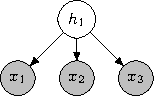
\includegraphics[width=0.95\textwidth,height=4cm,keepaspectratio]{figures/three-view.pdf} \\
      \includegraphics[width=0.95\textwidth,keepaspectratio]{figures/lhood.pdf}
    \end{figure}
    \vspace{-1cm}
  \begin{itemize}
    \item {\bf How can we apply the method of moments to consistently
      and efficiently estimate parameters for a general model family?}
  \end{itemize}
  }
\end{block}
\vfill

\begin{block}{Setup}
  \splitcolumn{%
    \begin{itemize}
      \item Assume discrete models with $k$ hidden and $d \ge k$
        observed values.
      \item Parameters and marginals can be represented as matrices
        and tensors.
      \item Presented in terms of infinite data and exact moments.
      \item Directed models are parameterized by their conditional
        probability tables.
      \item Undirected models are parameterized as a log-linear model,
        {\small
        \begin{align*}
        p(x) &= \exp(\sum_{\sC \in \sG} \theta^\top \phi(x_\sC, h_\sC) - A(\theta)).
        \end{align*}
        }
    \end{itemize}
 }{%
    \centering
    \begin{tikzpicture}
        % The model
        \point{start}{(0cm,0cm)}; %{pic cs:gen} -| mark)};
        % Matrices
        % - M12
        \node[scale=0.8] (m12) at ($(start) + (0.5cm,0.25cm)$) {\objw{3cm}{
          \begin{align*}
            M_{12} &\eqdef \Pr(x_1, x_2) \\
            {\color{blue} (M_{12})_{ij}} &\eqdef {\color{blue} \Pr(x_1 = i, x_2 = j)}
          \end{align*}
          }
        };
%        \point{m12c}{($(m12) + (1.5cm,0.75cm)$)};
         \tikzrect{m12r}{black,fill=white} {($(m12) + (3.2cm,0.75cm)$)}{1}{1};
         \tikzrect{m12ijr}{black,fill=blue}{($(m12) + (3.2cm,0.75cm)$)}{0.2}{0.2};
        % - M123
        \node[below=0.25cm of m12, scale=0.8] (m123) {\objw{3cm}{
          \begin{align*}
            M_{123} &\eqdef \Pr(x_1, x_2, x_3) \\
            {\color{blue} (M_{123})_{ijk}} &\eqdef {\color{blue} \Pr(x_1 = i, x_2 = j, x_3=k)}
          \end{align*}
          }
        };
%        \point{m123-c}{($(m123) + (1.75cm,0.75cm)$)};
        \tikzcube{m123r}{black,fill=white} {($(m123) + (3.2cm,0.75cm)$)}{1}{1}{1};
        \tikzcube{m123ijr}{black,fill=blue}{($(m123) + (3.2cm,0.75cm)$)}{0.2}{0.2}{0.2};

        % - O11
        \node[below=0.25cm of m123, scale=0.8] (o11) {\objw{3cm}{
          \begin{align*}
            \mOpp{1}{1} &\eqdef \Pr(x_1 \given h_1) \\
            {\color{DarkGreen} (\mOpp{1}{1})_{ij}} &\eqdef {\color{DarkGreen} \Pr(x_1 = i \given h_1 = j)}
          \end{align*}
          }
        };
%        \point{m123-c}{($(m123) + (1.75cm,0.75cm)$)};
        \tikzrect{o11r}{black,fill=white} {($(o11) + (3.2cm,0.75cm)$)}{1}{1};
        \tikzrect{o11ijr}{black,fill=DarkGreen}{($(o11) + (3.2cm,0.75cm)$)}{0.2}{0.2};
      \end{tikzpicture}
      \begin{tikzpicture}
        \point{stuff}{(2cm,0cm)};
        \drawbridge{(stuff)};
        \node[scale = 0.5, anchor=south] at (h1h2) {
          \begin{tabular}{r | l l}
            \diaghead{aaaaaa}{$h_2$}{$h_1$} &
            \thead{$0$} & \thead{$1$} \\ \hline 
            $0$ & \quad & \quad \\ 
            $1$ & \quad & \quad 
          \end{tabular}
        };
      \end{tikzpicture}
      \begin{tikzpicture}
        \point{stuff}{(2cm,0cm)};
        \drawubridge{(stuff)};
        \node[scale = 1.0, anchor=south] at (h1h2) {$\theta$};
      \end{tikzpicture}
  }
\end{block}
\vfill

\begin{block}{1. Bottlenecks}
  \splitcolumn{%
    \begin{itemize}
      \item A hidden variable $h$ is a {\bf bottleneck} if there exist three
        observed variables ({\bf views}) $x_1, x_2, x_3$ that are
        {\em conditionally independent} given $h$.
      \item We say a set of variables is {\em bottlenecked} if each
        variable is a bottleneck.
    \end{itemize}
  }{%
    \begin{itemize}
      \item \cite{anandkumar13tensor} provide an algorithm to estimate
        conditional moments $\Pr(x_i \given h)$ based on tensor
        eigendecomposition.
      \end{itemize}
  }
\end{block}
\vfill
\begin{block}{Limitations of bottlenecks}
  \splitcolumn{%
    \begin{itemize}
      \item Solving bottlenecks only provide conditional moments
        $\mOpp{1}{1} \eqdef \Pr(x_1 \given h_1)$. There are parameters
        that are not conditional moments. For example $\Pr(h_2 \given
        h_1)$ in the bridge model.
      \item {\bf An alternate approach:} fix the conditional moments;
        then the hidden marginals $Z_{12}$ and observed moments $M_{12}$
        are linearly related and can be solved.
      \item Main takeaway: Fixing conditional moments (learned using
        bottlenecks) simplifies learning other parameters.
    \end{itemize}
  }{%
  {
    \begin{figure}
    \centering
    \begin{tikzpicture}
    \point{mark}{(0,0)};
    \drawbridge{(mark)};
    \begin{pgfonlayer}{background}
    \draw[draw=black,fill=green!70,rounded corners,line width=1pt, dotted] 
                    ($(x1a.west) + (180:0.3cm)$) -- 
                    ($(h1.north) + (90:0.3cm)$) -- 
                    ($(x2a.east) + (0:0.3cm)$) -- 
                    ($(x2a.south) + (-90:0.3cm)$) -- 
                    ($(x1b.south) + (-90:0.3cm)$) -- 
                    ($(x1a.south) + (-90:0.3cm)$) -- 
                    cycle;
    \draw[dashed,-latex] (h1) -- (x2a);
    \end{pgfonlayer}
    \draw[-latex,DarkGreen] (h1) -- (x1a);
    \draw[-latex,DarkGreen] (h1) -- (x1b);

    \draw[-latex,DarkGreen,dashed] (h1) -- (x2a);

     \draw[-latex,DarkGreen] (h2) -- (x2a);
     \draw[-latex,DarkGreen] (h2) -- (x2b);
     \draw[-latex,DarkGreen,dashed] (h2) -- (x1b);

     \draw[-latex,red] (h1) -- (h2);
    \end{tikzpicture}
    \caption{The bridge model}
    \end{figure}
    }

    {\small
    \begin{align*}
      \underbrace{\Pr(x_1^b, x_2^a)}_{M_{12}} &= \sum_{h_1, h_2} 
      \underbrace{\Pr(x_1^b | h_1)}_{\mOpp{1}{1}}
      \underbrace{\Pr(x_2^a | h_2)}_{\mOpp{2}{2}}
      \underbrace{\Pr(h_1, h_2)}_{Z_{12}} \\
      M_{12} &= \mOpp{1}{1} Z_{12} \mOppt{2}{2} \\
      Z_{12} &= \mOppi{1}{1} M_{12} \mOppit{2}{2}
    \end{align*}
    }
  }
\end{block}

